% Options for packages loaded elsewhere
\PassOptionsToPackage{unicode}{hyperref}
\PassOptionsToPackage{hyphens}{url}
%
\documentclass[
]{article}
\usepackage{amsmath,amssymb}
\usepackage{iftex}
\ifPDFTeX
  \usepackage[T1]{fontenc}
  \usepackage[utf8]{inputenc}
  \usepackage{textcomp} % provide euro and other symbols
\else % if luatex or xetex
  \usepackage{unicode-math} % this also loads fontspec
  \defaultfontfeatures{Scale=MatchLowercase}
  \defaultfontfeatures[\rmfamily]{Ligatures=TeX,Scale=1}
\fi
\usepackage{lmodern}
\ifPDFTeX\else
  % xetex/luatex font selection
\fi
% Use upquote if available, for straight quotes in verbatim environments
\IfFileExists{upquote.sty}{\usepackage{upquote}}{}
\IfFileExists{microtype.sty}{% use microtype if available
  \usepackage[]{microtype}
  \UseMicrotypeSet[protrusion]{basicmath} % disable protrusion for tt fonts
}{}
\makeatletter
\@ifundefined{KOMAClassName}{% if non-KOMA class
  \IfFileExists{parskip.sty}{%
    \usepackage{parskip}
  }{% else
    \setlength{\parindent}{0pt}
    \setlength{\parskip}{6pt plus 2pt minus 1pt}}
}{% if KOMA class
  \KOMAoptions{parskip=half}}
\makeatother
\usepackage{xcolor}
\usepackage[margin=1in]{geometry}
\usepackage{color}
\usepackage{fancyvrb}
\newcommand{\VerbBar}{|}
\newcommand{\VERB}{\Verb[commandchars=\\\{\}]}
\DefineVerbatimEnvironment{Highlighting}{Verbatim}{commandchars=\\\{\}}
% Add ',fontsize=\small' for more characters per line
\usepackage{framed}
\definecolor{shadecolor}{RGB}{248,248,248}
\newenvironment{Shaded}{\begin{snugshade}}{\end{snugshade}}
\newcommand{\AlertTok}[1]{\textcolor[rgb]{0.94,0.16,0.16}{#1}}
\newcommand{\AnnotationTok}[1]{\textcolor[rgb]{0.56,0.35,0.01}{\textbf{\textit{#1}}}}
\newcommand{\AttributeTok}[1]{\textcolor[rgb]{0.13,0.29,0.53}{#1}}
\newcommand{\BaseNTok}[1]{\textcolor[rgb]{0.00,0.00,0.81}{#1}}
\newcommand{\BuiltInTok}[1]{#1}
\newcommand{\CharTok}[1]{\textcolor[rgb]{0.31,0.60,0.02}{#1}}
\newcommand{\CommentTok}[1]{\textcolor[rgb]{0.56,0.35,0.01}{\textit{#1}}}
\newcommand{\CommentVarTok}[1]{\textcolor[rgb]{0.56,0.35,0.01}{\textbf{\textit{#1}}}}
\newcommand{\ConstantTok}[1]{\textcolor[rgb]{0.56,0.35,0.01}{#1}}
\newcommand{\ControlFlowTok}[1]{\textcolor[rgb]{0.13,0.29,0.53}{\textbf{#1}}}
\newcommand{\DataTypeTok}[1]{\textcolor[rgb]{0.13,0.29,0.53}{#1}}
\newcommand{\DecValTok}[1]{\textcolor[rgb]{0.00,0.00,0.81}{#1}}
\newcommand{\DocumentationTok}[1]{\textcolor[rgb]{0.56,0.35,0.01}{\textbf{\textit{#1}}}}
\newcommand{\ErrorTok}[1]{\textcolor[rgb]{0.64,0.00,0.00}{\textbf{#1}}}
\newcommand{\ExtensionTok}[1]{#1}
\newcommand{\FloatTok}[1]{\textcolor[rgb]{0.00,0.00,0.81}{#1}}
\newcommand{\FunctionTok}[1]{\textcolor[rgb]{0.13,0.29,0.53}{\textbf{#1}}}
\newcommand{\ImportTok}[1]{#1}
\newcommand{\InformationTok}[1]{\textcolor[rgb]{0.56,0.35,0.01}{\textbf{\textit{#1}}}}
\newcommand{\KeywordTok}[1]{\textcolor[rgb]{0.13,0.29,0.53}{\textbf{#1}}}
\newcommand{\NormalTok}[1]{#1}
\newcommand{\OperatorTok}[1]{\textcolor[rgb]{0.81,0.36,0.00}{\textbf{#1}}}
\newcommand{\OtherTok}[1]{\textcolor[rgb]{0.56,0.35,0.01}{#1}}
\newcommand{\PreprocessorTok}[1]{\textcolor[rgb]{0.56,0.35,0.01}{\textit{#1}}}
\newcommand{\RegionMarkerTok}[1]{#1}
\newcommand{\SpecialCharTok}[1]{\textcolor[rgb]{0.81,0.36,0.00}{\textbf{#1}}}
\newcommand{\SpecialStringTok}[1]{\textcolor[rgb]{0.31,0.60,0.02}{#1}}
\newcommand{\StringTok}[1]{\textcolor[rgb]{0.31,0.60,0.02}{#1}}
\newcommand{\VariableTok}[1]{\textcolor[rgb]{0.00,0.00,0.00}{#1}}
\newcommand{\VerbatimStringTok}[1]{\textcolor[rgb]{0.31,0.60,0.02}{#1}}
\newcommand{\WarningTok}[1]{\textcolor[rgb]{0.56,0.35,0.01}{\textbf{\textit{#1}}}}
\usepackage{graphicx}
\makeatletter
\def\maxwidth{\ifdim\Gin@nat@width>\linewidth\linewidth\else\Gin@nat@width\fi}
\def\maxheight{\ifdim\Gin@nat@height>\textheight\textheight\else\Gin@nat@height\fi}
\makeatother
% Scale images if necessary, so that they will not overflow the page
% margins by default, and it is still possible to overwrite the defaults
% using explicit options in \includegraphics[width, height, ...]{}
\setkeys{Gin}{width=\maxwidth,height=\maxheight,keepaspectratio}
% Set default figure placement to htbp
\makeatletter
\def\fps@figure{htbp}
\makeatother
\setlength{\emergencystretch}{3em} % prevent overfull lines
\providecommand{\tightlist}{%
  \setlength{\itemsep}{0pt}\setlength{\parskip}{0pt}}
\setcounter{secnumdepth}{-\maxdimen} % remove section numbering
\ifLuaTeX
  \usepackage{selnolig}  % disable illegal ligatures
\fi
\IfFileExists{bookmark.sty}{\usepackage{bookmark}}{\usepackage{hyperref}}
\IfFileExists{xurl.sty}{\usepackage{xurl}}{} % add URL line breaks if available
\urlstyle{same}
\hypersetup{
  pdftitle={Exploring R},
  hidelinks,
  pdfcreator={LaTeX via pandoc}}

\title{Exploring R}
\author{}
\date{\vspace{-2.5em}2023-11-01}

\begin{document}
\maketitle

\begin{Shaded}
\begin{Highlighting}[]
\FunctionTok{library}\NormalTok{(here)}
\end{Highlighting}
\end{Shaded}

\begin{verbatim}
## here() starts at C:/Users/Blake/Dropbox/My PC (LAPTOP-R53ILDBG)/Documents/GitHub/Terzan-5
\end{verbatim}

\begin{Shaded}
\begin{Highlighting}[]
\NormalTok{here}\SpecialCharTok{::}\FunctionTok{i\_am}\NormalTok{(}\StringTok{"Functions of R.Rmd"}\NormalTok{)}
\end{Highlighting}
\end{Shaded}

\begin{verbatim}
## here() starts at C:/Users/Blake/Dropbox/My PC (LAPTOP-R53ILDBG)/Documents/GitHub/Terzan-5
\end{verbatim}

\begin{Shaded}
\begin{Highlighting}[]
\FunctionTok{here}\NormalTok{()}
\end{Highlighting}
\end{Shaded}

\begin{verbatim}
## [1] "C:/Users/Blake/Dropbox/My PC (LAPTOP-R53ILDBG)/Documents/GitHub/Terzan-5"
\end{verbatim}

\begin{Shaded}
\begin{Highlighting}[]
\FunctionTok{here}\NormalTok{()}
\end{Highlighting}
\end{Shaded}

\begin{verbatim}
## [1] "C:/Users/Blake/Dropbox/My PC (LAPTOP-R53ILDBG)/Documents/GitHub/Terzan-5"
\end{verbatim}

\begin{Shaded}
\begin{Highlighting}[]
\NormalTok{Tz5 }\OtherTok{\textless{}{-}}\NormalTok{ readr}\SpecialCharTok{::}\FunctionTok{read\_csv}\NormalTok{(}\FunctionTok{here}\NormalTok{(}\StringTok{"Data"}\NormalTok{, }\StringTok{"Terzan 5 X{-}ray events.csv"}\NormalTok{), }\AttributeTok{col\_types =} \FunctionTok{list}\NormalTok{(}\AttributeTok{.default =}\NormalTok{ readr}\SpecialCharTok{::}\FunctionTok{col\_guess}\NormalTok{()), )}
\end{Highlighting}
\end{Shaded}

\begin{Shaded}
\begin{Highlighting}[]
\FunctionTok{library}\NormalTok{(ggplot2)}
\FunctionTok{library}\NormalTok{(plotly)}
\end{Highlighting}
\end{Shaded}

\begin{verbatim}
## 
## Attaching package: 'plotly'
\end{verbatim}

\begin{verbatim}
## The following object is masked from 'package:ggplot2':
## 
##     last_plot
\end{verbatim}

\begin{verbatim}
## The following object is masked from 'package:stats':
## 
##     filter
\end{verbatim}

\begin{verbatim}
## The following object is masked from 'package:graphics':
## 
##     layout
\end{verbatim}

\begin{Shaded}
\begin{Highlighting}[]
\FunctionTok{library}\NormalTok{(readr)}
\FunctionTok{library}\NormalTok{(ggpointdensity)}
\FunctionTok{library}\NormalTok{(viridis)}
\end{Highlighting}
\end{Shaded}

\begin{verbatim}
## Loading required package: viridisLite
\end{verbatim}

\begin{Shaded}
\begin{Highlighting}[]
\FunctionTok{library}\NormalTok{(tidyr)}
\FunctionTok{library}\NormalTok{(fitdistrplus)}
\end{Highlighting}
\end{Shaded}

\begin{verbatim}
## Loading required package: MASS
\end{verbatim}

\begin{verbatim}
## 
## Attaching package: 'MASS'
\end{verbatim}

\begin{verbatim}
## The following object is masked from 'package:plotly':
## 
##     select
\end{verbatim}

\begin{verbatim}
## Loading required package: survival
\end{verbatim}

\begin{Shaded}
\begin{Highlighting}[]
\NormalTok{T5 }\OtherTok{\textless{}{-}} \FunctionTok{data.frame}\NormalTok{(Tz5}\SpecialCharTok{$}\NormalTok{x, Tz5}\SpecialCharTok{$}\NormalTok{y)}
\FunctionTok{colnames}\NormalTok{(T5) }\OtherTok{\textless{}{-}} \FunctionTok{c}\NormalTok{(}\StringTok{\textquotesingle{}x\textquotesingle{}}\NormalTok{,}\StringTok{\textquotesingle{}y\textquotesingle{}}\NormalTok{)}
\NormalTok{POI1 }\OtherTok{\textless{}{-}}\NormalTok{ T5 }\SpecialCharTok{\%\textgreater{}\%}
  \FunctionTok{filter}\NormalTok{(x}\SpecialCharTok{\textgreater{}}\DecValTok{4160} \SpecialCharTok{\&}\NormalTok{ x}\SpecialCharTok{\textless{}}\DecValTok{4180} \SpecialCharTok{\&}\NormalTok{ y}\SpecialCharTok{\textgreater{}}\DecValTok{4180} \SpecialCharTok{\&}\NormalTok{ y}\SpecialCharTok{\textless{}}\DecValTok{4200}\NormalTok{)}
\NormalTok{POI2 }\OtherTok{\textless{}{-}}\NormalTok{ T5 }\SpecialCharTok{\%\textgreater{}\%}
  \FunctionTok{filter}\NormalTok{(x}\SpecialCharTok{\textgreater{}}\DecValTok{4105} \SpecialCharTok{\&}\NormalTok{ x}\SpecialCharTok{\textless{}} \DecValTok{4125} \SpecialCharTok{\&}\NormalTok{ y}\SpecialCharTok{\textgreater{}}\DecValTok{4040} \SpecialCharTok{\&}\NormalTok{ y}\SpecialCharTok{\textless{}}\DecValTok{4060}\NormalTok{)}
\NormalTok{Central }\OtherTok{\textless{}{-}}\NormalTok{ T5 }\SpecialCharTok{\%\textgreater{}\%}
  \FunctionTok{filter}\NormalTok{(x}\SpecialCharTok{\textgreater{}}\DecValTok{4085} \SpecialCharTok{\&}\NormalTok{ x}\SpecialCharTok{\textless{}} \DecValTok{4150} \SpecialCharTok{\&}\NormalTok{ y}\SpecialCharTok{\textgreater{}}\DecValTok{4060} \SpecialCharTok{\&}\NormalTok{ y}\SpecialCharTok{\textless{}}\DecValTok{4125}\NormalTok{)}
\NormalTok{POI3 }\OtherTok{\textless{}{-}}\NormalTok{ T5 }\SpecialCharTok{\%\textgreater{}\%}
  \FunctionTok{filter}\NormalTok{(x}\SpecialCharTok{\textgreater{}}\DecValTok{4120} \SpecialCharTok{\&}\NormalTok{ x}\SpecialCharTok{\textless{}} \DecValTok{4140} \SpecialCharTok{\&}\NormalTok{ y}\SpecialCharTok{\textgreater{}}\DecValTok{4100} \SpecialCharTok{\&}\NormalTok{ y}\SpecialCharTok{\textless{}}\DecValTok{4120}\NormalTok{)}

\NormalTok{dMoffat1D }\OtherTok{\textless{}{-}} \ControlFlowTok{function}\NormalTok{(x, amplitude, mu, gamma, alpha)\{amplitude}\SpecialCharTok{*}\NormalTok{(}\DecValTok{1}\SpecialCharTok{+}\NormalTok{((x}\SpecialCharTok{{-}}\NormalTok{mu)}\SpecialCharTok{/}\NormalTok{gamma)}\SpecialCharTok{\^{}}\DecValTok{2}\NormalTok{)}\SpecialCharTok{\^{}{-}}\NormalTok{alpha\}}

\NormalTok{Moffat1D\_Deriv }\OtherTok{\textless{}{-}} \ControlFlowTok{function}\NormalTok{(x, amplitude, mu, gamma, alpha)\{}
\NormalTok{  chain }\OtherTok{=}\NormalTok{ (}\DecValTok{1} \SpecialCharTok{+}\NormalTok{ (x }\SpecialCharTok{{-}}\NormalTok{ mu)}\SpecialCharTok{\^{}}\DecValTok{2} \SpecialCharTok{/}\NormalTok{ gamma}\SpecialCharTok{\^{}}\DecValTok{2}\NormalTok{)}
\NormalTok{  d\_A }\OtherTok{=}\NormalTok{ chain}\SpecialCharTok{\^{}}\NormalTok{(}\SpecialCharTok{{-}}\NormalTok{alpha)}
\NormalTok{  d\_mu }\OtherTok{=} \DecValTok{2}\SpecialCharTok{*}\NormalTok{amplitude}\SpecialCharTok{*}\NormalTok{alpha}\SpecialCharTok{*}\NormalTok{(x }\SpecialCharTok{{-}}\NormalTok{ mu)}\SpecialCharTok{*}\NormalTok{d\_A}\SpecialCharTok{/}\NormalTok{(chain}\SpecialCharTok{*}\NormalTok{gamma}\SpecialCharTok{\^{}}\DecValTok{2}\NormalTok{)}
\NormalTok{  d\_gamma }\OtherTok{=} \DecValTok{2}\SpecialCharTok{*}\NormalTok{amplitude}\SpecialCharTok{*}\NormalTok{alpha}\SpecialCharTok{*}\NormalTok{((x }\SpecialCharTok{{-}}\NormalTok{ mu)}\SpecialCharTok{\^{}}\DecValTok{2}\NormalTok{)}\SpecialCharTok{*}\NormalTok{d\_A}\SpecialCharTok{/}\NormalTok{(chain}\SpecialCharTok{*}\NormalTok{gamma}\SpecialCharTok{\^{}}\DecValTok{3}\NormalTok{)}
\NormalTok{  d\_alpha }\OtherTok{=} \SpecialCharTok{{-}}\NormalTok{amplitude}\SpecialCharTok{*}\NormalTok{d\_A}\SpecialCharTok{*}\FunctionTok{log}\NormalTok{(chain)}
  
  \FunctionTok{return}\NormalTok{(}\FunctionTok{list}\NormalTok{(}\FunctionTok{c}\NormalTok{(d\_A, d\_mu, d\_gamma, d\_alpha)))}
\NormalTok{\}}
\end{Highlighting}
\end{Shaded}

\begin{Shaded}
\begin{Highlighting}[]
\FunctionTok{set.seed}\NormalTok{(}\DecValTok{0}\NormalTok{)}
\NormalTok{g1 }\OtherTok{\textless{}{-}} \FunctionTok{rgamma}\NormalTok{(}\DecValTok{1000}\NormalTok{, }\AttributeTok{shape =} \DecValTok{2}\NormalTok{, }\AttributeTok{rate =} \DecValTok{1}\NormalTok{)}

\FunctionTok{set.seed}\NormalTok{(}\DecValTok{1}\NormalTok{)}
\NormalTok{g2 }\OtherTok{\textless{}{-}} \FunctionTok{rgamma}\NormalTok{(}\DecValTok{1000}\NormalTok{, }\AttributeTok{shape =} \DecValTok{10}\NormalTok{, }\AttributeTok{rate =} \DecValTok{1}\NormalTok{)}

\FunctionTok{set.seed}\NormalTok{(}\DecValTok{2}\NormalTok{)}
\NormalTok{g3 }\OtherTok{\textless{}{-}} \FunctionTok{rgamma}\NormalTok{(}\DecValTok{1000}\NormalTok{, }\AttributeTok{shape =} \DecValTok{2}\NormalTok{, }\AttributeTok{rate =} \DecValTok{10}\NormalTok{)}

\FunctionTok{set.seed}\NormalTok{(}\DecValTok{3}\NormalTok{)}
\NormalTok{g4 }\OtherTok{\textless{}{-}} \FunctionTok{rgamma}\NormalTok{(}\DecValTok{1000}\NormalTok{, }\AttributeTok{shape =} \DecValTok{10}\NormalTok{, }\AttributeTok{rate =} \DecValTok{10}\NormalTok{)}

\FunctionTok{par}\NormalTok{(}\AttributeTok{mfrow =} \FunctionTok{c}\NormalTok{(}\DecValTok{2}\NormalTok{,}\DecValTok{2}\NormalTok{))}
\FunctionTok{hist}\NormalTok{(g1)}
\FunctionTok{hist}\NormalTok{(g2)}
\FunctionTok{hist}\NormalTok{(g3)}
\FunctionTok{hist}\NormalTok{(g4)}
\end{Highlighting}
\end{Shaded}

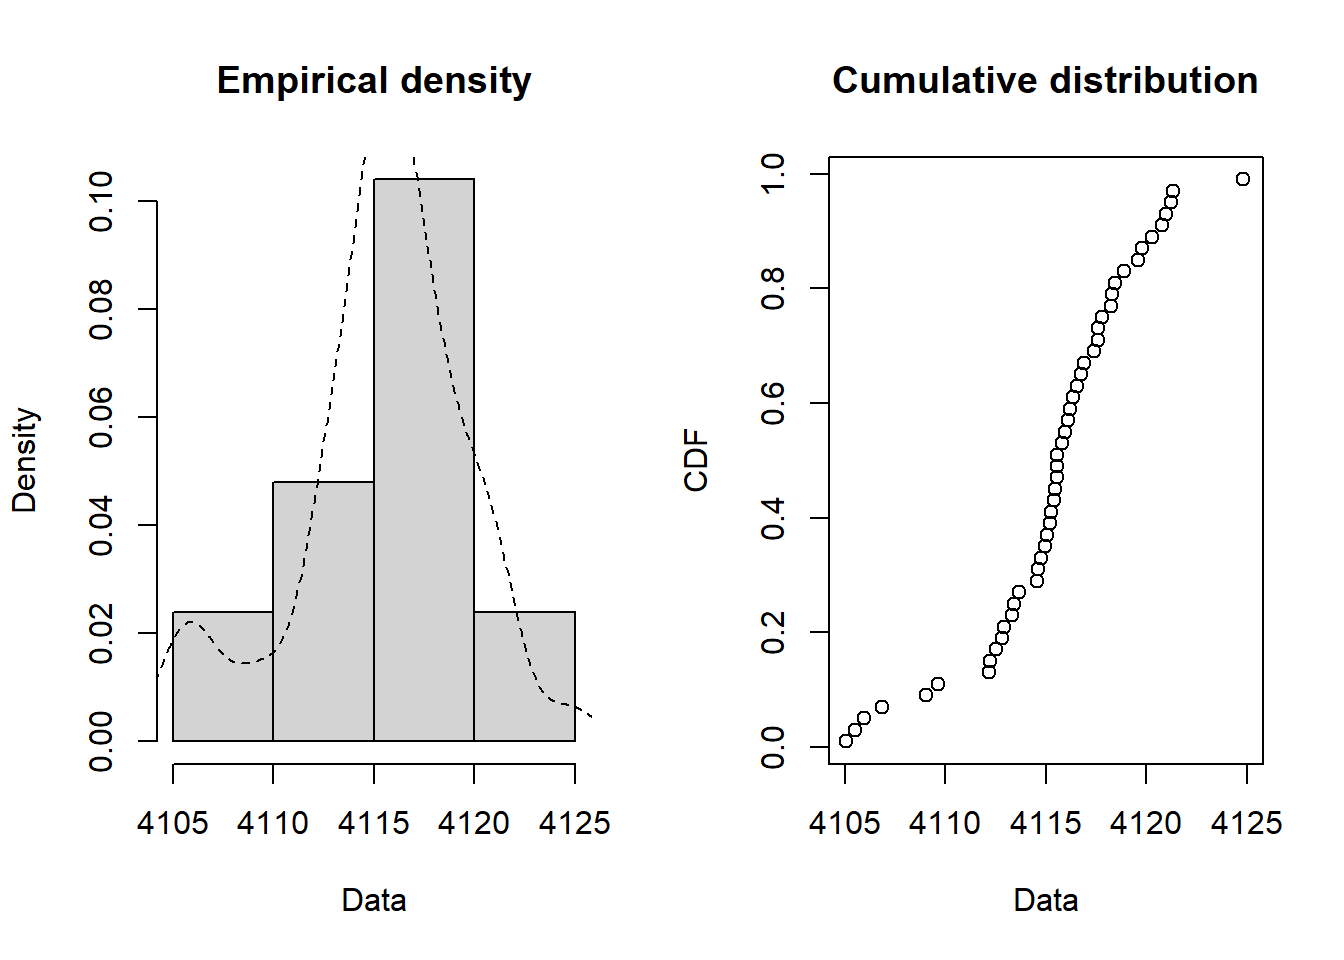
\includegraphics{Functions-of-R_files/figure-latex/unnamed-chunk-5-1.pdf}

\begin{Shaded}
\begin{Highlighting}[]
\CommentTok{\#Moffat 1D}
\CommentTok{\#One Dimensional Moffat Model}

\CommentTok{\#Model Formula}
\CommentTok{\#f(x) = A(1+(x{-}mu)\^{}2/gamma\^{}2)\^{}{-}alpha}

\CommentTok{\#Parameters}
\CommentTok{\#A = Amplitude}
\CommentTok{\#mu = the x position of the maximum of the model }
\CommentTok{\#gamma = core width of the model}
\CommentTok{\#alpha = power index}

\CommentTok{\#Defaults}
\CommentTok{\#Amplitude = 1}
\CommentTok{\#mu = 0}
\CommentTok{\#gamma = 1}
\CommentTok{\#alpha = 1}

\NormalTok{dMoffat1D }\OtherTok{\textless{}{-}} \ControlFlowTok{function}\NormalTok{(x, amplitude, mu, gamma, alpha)\{amplitude}\SpecialCharTok{*}\NormalTok{(}\DecValTok{1}\SpecialCharTok{+}\NormalTok{((x}\SpecialCharTok{{-}}\NormalTok{mu)}\SpecialCharTok{/}\NormalTok{gamma)}\SpecialCharTok{\^{}}\DecValTok{2}\NormalTok{)}\SpecialCharTok{\^{}{-}}\NormalTok{alpha\}}

\NormalTok{Moffat1D\_Deriv }\OtherTok{\textless{}{-}} \ControlFlowTok{function}\NormalTok{(x, amplitude, mu, gamma, alpha)\{}
\NormalTok{  chain }\OtherTok{=}\NormalTok{ (}\DecValTok{1} \SpecialCharTok{+}\NormalTok{ (x }\SpecialCharTok{{-}}\NormalTok{ mu)}\SpecialCharTok{\^{}}\DecValTok{2} \SpecialCharTok{/}\NormalTok{ gamma}\SpecialCharTok{\^{}}\DecValTok{2}\NormalTok{)}
\NormalTok{  d\_A }\OtherTok{=}\NormalTok{ chain}\SpecialCharTok{\^{}}\NormalTok{(}\SpecialCharTok{{-}}\NormalTok{alpha)}
\NormalTok{  d\_mu }\OtherTok{=} \DecValTok{2}\SpecialCharTok{*}\NormalTok{amplitude}\SpecialCharTok{*}\NormalTok{alpha}\SpecialCharTok{*}\NormalTok{(x }\SpecialCharTok{{-}}\NormalTok{ mu)}\SpecialCharTok{*}\NormalTok{d\_A}\SpecialCharTok{/}\NormalTok{(chain}\SpecialCharTok{*}\NormalTok{gamma}\SpecialCharTok{\^{}}\DecValTok{2}\NormalTok{)}
\NormalTok{  d\_gamma }\OtherTok{=} \DecValTok{2}\SpecialCharTok{*}\NormalTok{amplitude}\SpecialCharTok{*}\NormalTok{alpha}\SpecialCharTok{*}\NormalTok{((x }\SpecialCharTok{{-}}\NormalTok{ mu)}\SpecialCharTok{\^{}}\DecValTok{2}\NormalTok{)}\SpecialCharTok{*}\NormalTok{d\_A}\SpecialCharTok{/}\NormalTok{(chain}\SpecialCharTok{*}\NormalTok{gamma}\SpecialCharTok{\^{}}\DecValTok{3}\NormalTok{)}
\NormalTok{  d\_alpha }\OtherTok{=} \SpecialCharTok{{-}}\NormalTok{amplitude}\SpecialCharTok{*}\NormalTok{d\_A}\SpecialCharTok{*}\FunctionTok{log}\NormalTok{(chain)}
  
  \FunctionTok{return}\NormalTok{(}\FunctionTok{list}\NormalTok{(}\FunctionTok{c}\NormalTok{(d\_A, d\_mu, d\_gamma, d\_alpha)))}
\NormalTok{\}}
\end{Highlighting}
\end{Shaded}

\begin{Shaded}
\begin{Highlighting}[]
\FunctionTok{set.seed}\NormalTok{(}\DecValTok{8}\NormalTok{)}

\NormalTok{randata }\OtherTok{\textless{}{-}} \FunctionTok{rgamma}\NormalTok{(}\DecValTok{1000}\NormalTok{, }\DecValTok{9}\NormalTok{, }\DecValTok{2}\NormalTok{)}
\FunctionTok{plot}\NormalTok{(randata)}
\end{Highlighting}
\end{Shaded}

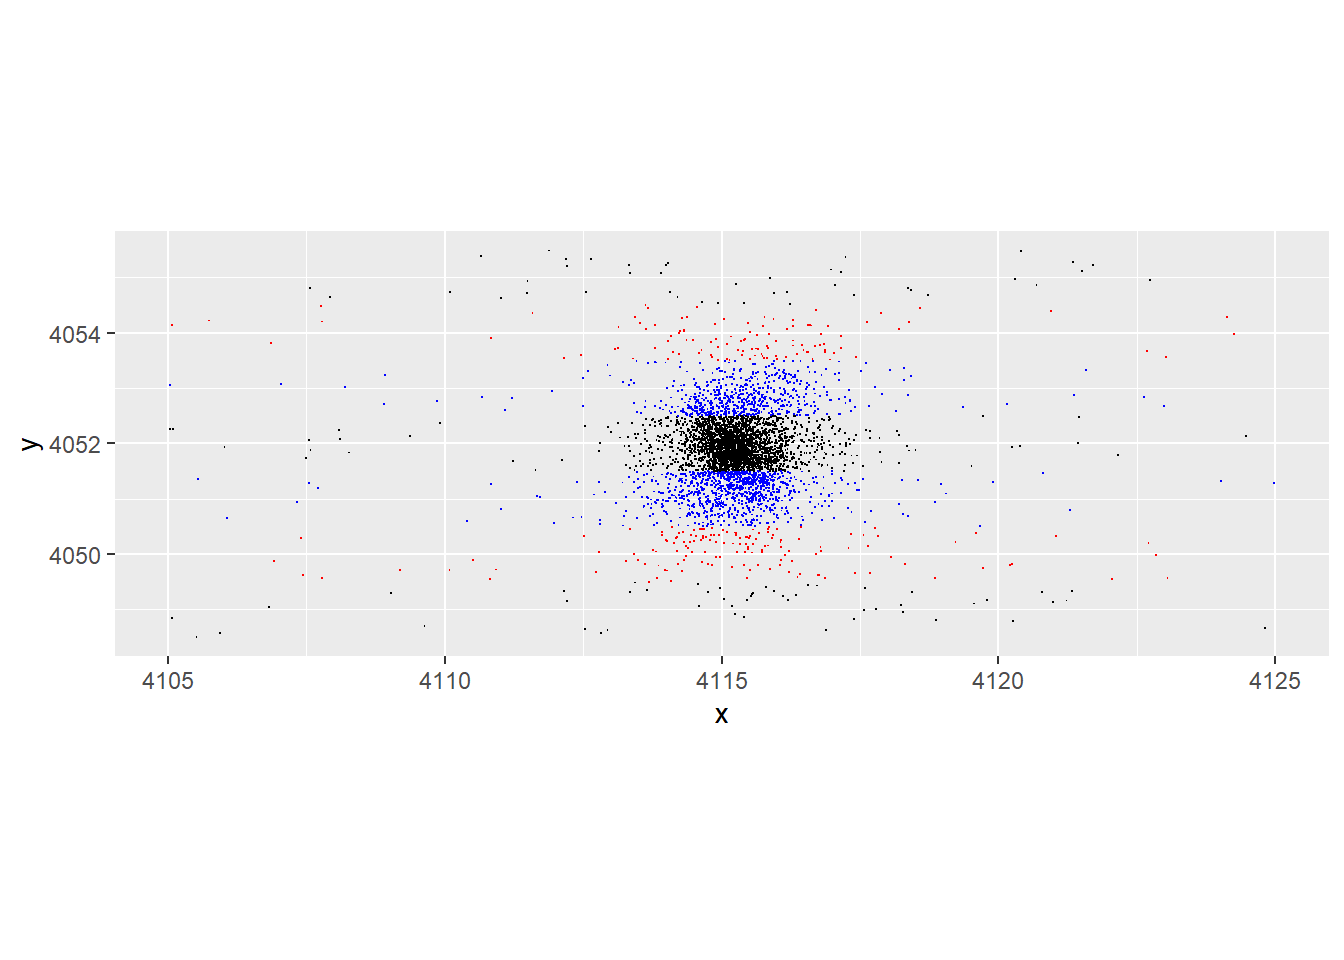
\includegraphics{Functions-of-R_files/figure-latex/unnamed-chunk-7-1.pdf}

\begin{Shaded}
\begin{Highlighting}[]
\FunctionTok{hist}\NormalTok{(randata)}
\end{Highlighting}
\end{Shaded}

\includegraphics{Functions-of-R_files/figure-latex/unnamed-chunk-7-2.pdf}

\begin{Shaded}
\begin{Highlighting}[]
\NormalTok{beta }\OtherTok{=} \DecValTok{2}
\NormalTok{alpha }\OtherTok{=} \DecValTok{9}
\end{Highlighting}
\end{Shaded}

\begin{Shaded}
\begin{Highlighting}[]
\NormalTok{Gamma }\OtherTok{\textless{}{-}} \ControlFlowTok{function}\NormalTok{(x, alpha, beta)\{}
\NormalTok{  ((beta}\SpecialCharTok{\^{}}\NormalTok{alpha)}\SpecialCharTok{/}\FunctionTok{factorial}\NormalTok{(alpha}\DecValTok{{-}1}\NormalTok{))}\SpecialCharTok{*}\NormalTok{ x}\SpecialCharTok{\^{}}\NormalTok{(alpha}\DecValTok{{-}1}\NormalTok{)}\SpecialCharTok{*} \FunctionTok{exp}\NormalTok{(}\SpecialCharTok{{-}}\NormalTok{beta}\SpecialCharTok{*}\NormalTok{x)}
\NormalTok{\}}

\NormalTok{range }\OtherTok{\textless{}{-}} \FunctionTok{seq}\NormalTok{(}\DecValTok{0}\NormalTok{,}\DecValTok{25}\NormalTok{, }\AttributeTok{by=}\FloatTok{0.1}\NormalTok{)}


\FunctionTok{plot}\NormalTok{(}\FunctionTok{Gamma}\NormalTok{(range, }\DecValTok{9}\NormalTok{, }\DecValTok{2}\NormalTok{))}
\end{Highlighting}
\end{Shaded}

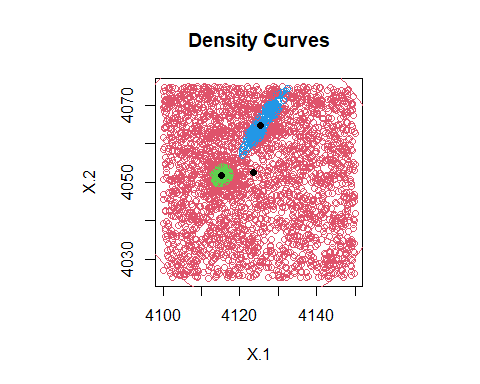
\includegraphics{Functions-of-R_files/figure-latex/unnamed-chunk-8-1.pdf}

\begin{Shaded}
\begin{Highlighting}[]
\FunctionTok{plotdist}\NormalTok{(randata, }\AttributeTok{demp =} \ConstantTok{TRUE}\NormalTok{)}
\end{Highlighting}
\end{Shaded}

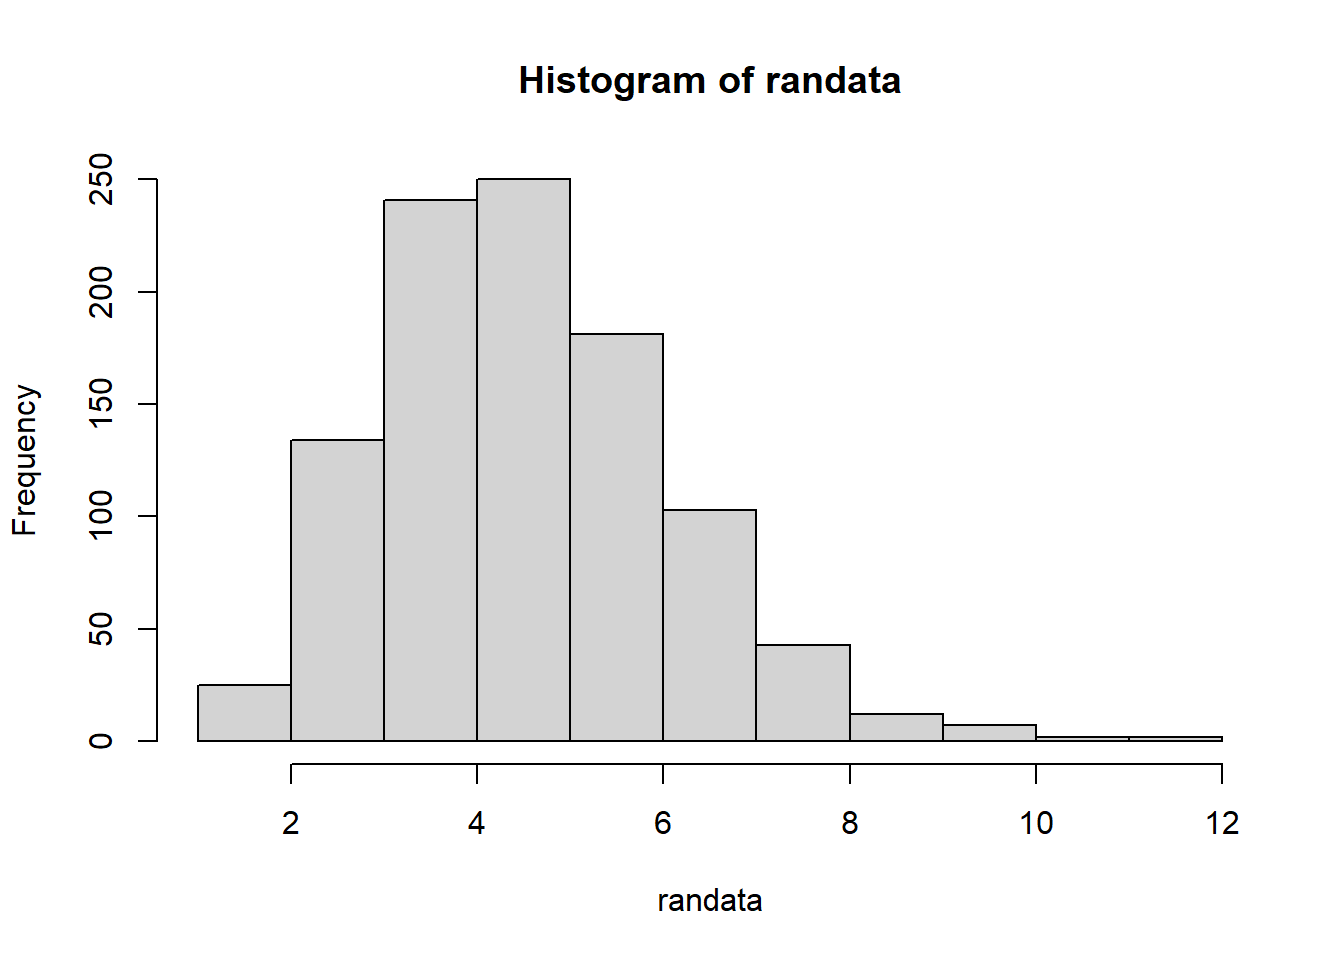
\includegraphics{Functions-of-R_files/figure-latex/unnamed-chunk-8-2.pdf}

\begin{Shaded}
\begin{Highlighting}[]
\CommentTok{\#check}
\FunctionTok{Gamma}\NormalTok{(}\DecValTok{5}\NormalTok{, }\DecValTok{9}\NormalTok{, }\DecValTok{2}\NormalTok{)}
\end{Highlighting}
\end{Shaded}

\begin{verbatim}
## [1] 0.2251981
\end{verbatim}

\begin{Shaded}
\begin{Highlighting}[]
\FunctionTok{dgamma}\NormalTok{(}\DecValTok{5}\NormalTok{, }\DecValTok{9}\NormalTok{, }\DecValTok{2}\NormalTok{)}
\end{Highlighting}
\end{Shaded}

\begin{verbatim}
## [1] 0.2251981
\end{verbatim}

\begin{Shaded}
\begin{Highlighting}[]
\CommentTok{\#res \textless{}{-} optim(c(5,9,2), Gamma)}
\end{Highlighting}
\end{Shaded}

\begin{Shaded}
\begin{Highlighting}[]
\CommentTok{\#optim example code}
\DocumentationTok{\#\# "wild" function , global minimum at about {-}15.81515}
\NormalTok{fw }\OtherTok{\textless{}{-}} \ControlFlowTok{function}\NormalTok{ (x)}
    \DecValTok{10}\SpecialCharTok{*}\FunctionTok{sin}\NormalTok{(}\FloatTok{0.3}\SpecialCharTok{*}\NormalTok{x)}\SpecialCharTok{*}\FunctionTok{sin}\NormalTok{(}\FloatTok{1.3}\SpecialCharTok{*}\NormalTok{x}\SpecialCharTok{\^{}}\DecValTok{2}\NormalTok{) }\SpecialCharTok{+} \FloatTok{0.00001}\SpecialCharTok{*}\NormalTok{x}\SpecialCharTok{\^{}}\DecValTok{4} \SpecialCharTok{+} \FloatTok{0.2}\SpecialCharTok{*}\NormalTok{x}\SpecialCharTok{+}\DecValTok{80}
\FunctionTok{plot}\NormalTok{(fw, }\SpecialCharTok{{-}}\DecValTok{50}\NormalTok{, }\DecValTok{50}\NormalTok{, }\AttributeTok{n =} \DecValTok{1000}\NormalTok{, }\AttributeTok{main =} \StringTok{"optim() minimising \textquotesingle{}wild function\textquotesingle{}"}\NormalTok{)}
\end{Highlighting}
\end{Shaded}

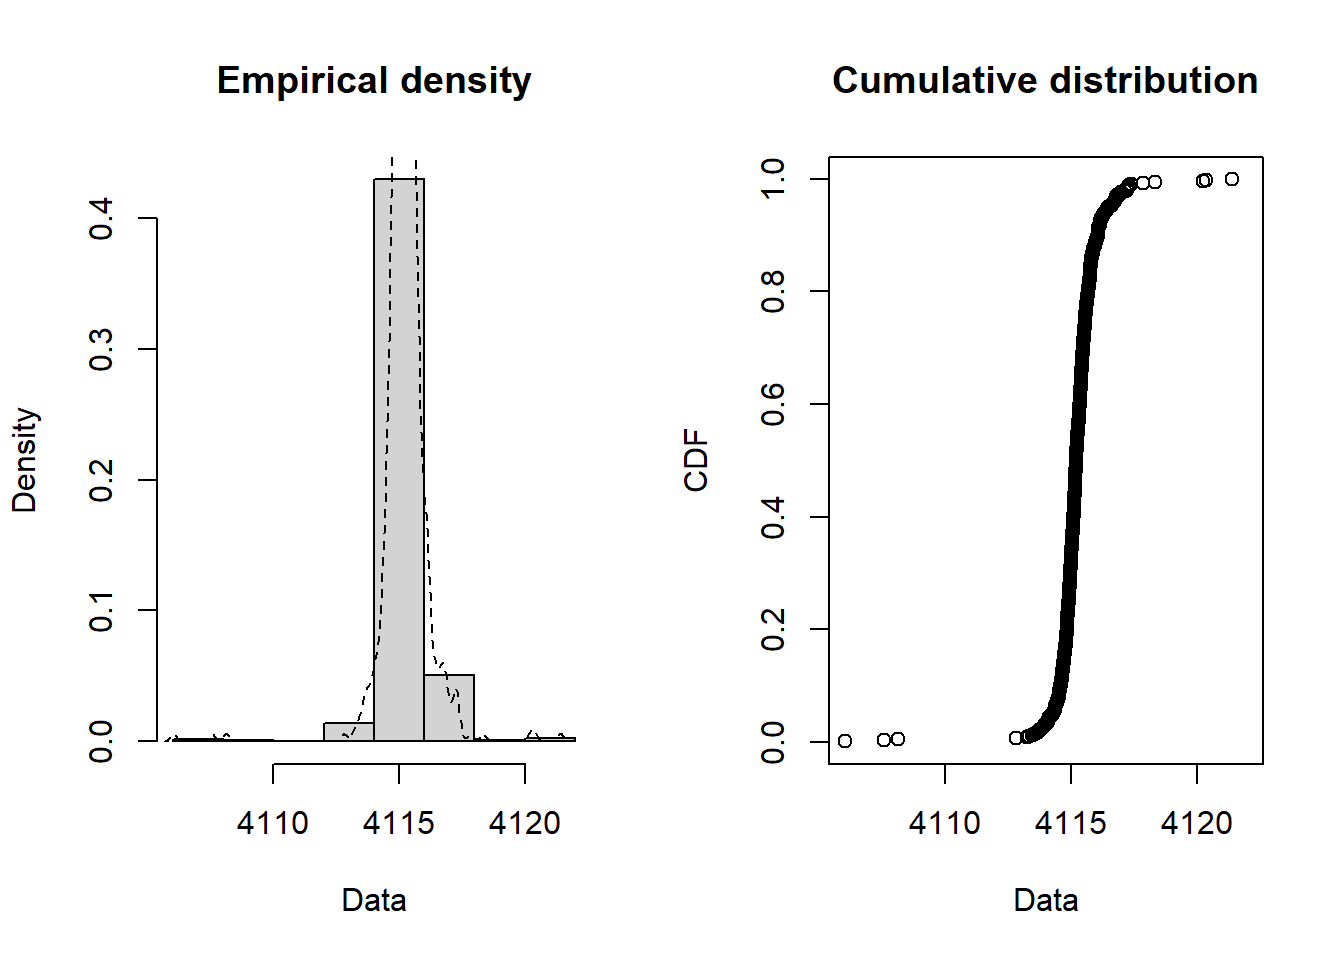
\includegraphics{Functions-of-R_files/figure-latex/unnamed-chunk-9-1.pdf}

\begin{Shaded}
\begin{Highlighting}[]
\NormalTok{res }\OtherTok{\textless{}{-}} \FunctionTok{optim}\NormalTok{(}\DecValTok{50}\NormalTok{, fw, }\AttributeTok{method =} \StringTok{"SANN"}\NormalTok{,}
             \AttributeTok{control =} \FunctionTok{list}\NormalTok{(}\AttributeTok{maxit =} \DecValTok{20000}\NormalTok{, }\AttributeTok{temp =} \DecValTok{20}\NormalTok{, }\AttributeTok{parscale =} \DecValTok{20}\NormalTok{))}
\NormalTok{res}
\end{Highlighting}
\end{Shaded}

\begin{verbatim}
## $par
## [1] -15.81461
## 
## $value
## [1] 67.47023
## 
## $counts
## function gradient 
##    20000       NA 
## 
## $convergence
## [1] 0
## 
## $message
## NULL
\end{verbatim}

\begin{Shaded}
\begin{Highlighting}[]
\NormalTok{range2 }\OtherTok{\textless{}{-}} \FunctionTok{seq}\NormalTok{(}\SpecialCharTok{{-}}\DecValTok{3}\NormalTok{, }\DecValTok{3}\NormalTok{, }\AttributeTok{by =} \FloatTok{0.1}\NormalTok{)}

\FunctionTok{par}\NormalTok{(}\AttributeTok{mfrow =} \FunctionTok{c}\NormalTok{(}\DecValTok{2}\NormalTok{,}\DecValTok{3}\NormalTok{))}
\FunctionTok{plot}\NormalTok{(}\FunctionTok{dMoffat1D}\NormalTok{(range2, }\DecValTok{1}\NormalTok{, }\DecValTok{0}\NormalTok{, }\DecValTok{1}\NormalTok{, }\DecValTok{1}\NormalTok{), }\AttributeTok{main =} \StringTok{"Default parameters"}\NormalTok{)}
\FunctionTok{plot}\NormalTok{(}\FunctionTok{dMoffat1D}\NormalTok{(range2, }\DecValTok{1}\NormalTok{, }\DecValTok{0}\NormalTok{, }\DecValTok{1}\NormalTok{, }\DecValTok{2}\NormalTok{), }\AttributeTok{main =} \StringTok{"Changing alpha"}\NormalTok{)}
\FunctionTok{plot}\NormalTok{(}\FunctionTok{dMoffat1D}\NormalTok{(range2, }\DecValTok{1}\NormalTok{, }\DecValTok{1}\NormalTok{, }\DecValTok{1}\NormalTok{, }\DecValTok{1}\NormalTok{), }\AttributeTok{main =} \StringTok{"Changing mu"}\NormalTok{)}
\FunctionTok{plot}\NormalTok{(}\FunctionTok{dMoffat1D}\NormalTok{(range2, }\DecValTok{1}\NormalTok{, }\DecValTok{0}\NormalTok{, }\FloatTok{0.5}\NormalTok{, }\DecValTok{1}\NormalTok{), }\AttributeTok{main =} \StringTok{"Changing gamma"}\NormalTok{)}
\FunctionTok{plot}\NormalTok{(}\FunctionTok{dMoffat1D}\NormalTok{(range2, }\DecValTok{4}\NormalTok{, }\DecValTok{0}\NormalTok{, }\DecValTok{1}\NormalTok{, }\DecValTok{1}\NormalTok{), }\AttributeTok{main =} \StringTok{"Changing A"}\NormalTok{)}
\FunctionTok{plot}\NormalTok{(}\FunctionTok{dMoffat1D}\NormalTok{(range2, }\DecValTok{4}\NormalTok{, }\DecValTok{1}\NormalTok{, }\DecValTok{4}\NormalTok{, }\DecValTok{4}\NormalTok{), }\AttributeTok{main =} \StringTok{"Changing all"}\NormalTok{)}
\end{Highlighting}
\end{Shaded}

\includegraphics{Functions-of-R_files/figure-latex/unnamed-chunk-10-1.pdf}

\begin{Shaded}
\begin{Highlighting}[]
\CommentTok{\# Define the Gaussian density function}
\NormalTok{gaussian\_density }\OtherTok{\textless{}{-}} \ControlFlowTok{function}\NormalTok{(x, mean, sd) \{}
  \FunctionTok{return}\NormalTok{(}\FunctionTok{dnorm}\NormalTok{(x, }\AttributeTok{mean =}\NormalTok{ mean, }\AttributeTok{sd =}\NormalTok{ sd))}
\NormalTok{\}}

\CommentTok{\# Define the negative log{-}likelihood function for Gaussian distribution}
\NormalTok{negative\_log\_likelihood }\OtherTok{\textless{}{-}} \ControlFlowTok{function}\NormalTok{(parameters, x) \{}
\NormalTok{  mean }\OtherTok{\textless{}{-}}\NormalTok{ parameters[}\DecValTok{1}\NormalTok{]}
\NormalTok{  sd }\OtherTok{\textless{}{-}}\NormalTok{ parameters[}\DecValTok{2}\NormalTok{]}
  
\NormalTok{  predicted\_density }\OtherTok{\textless{}{-}} \FunctionTok{gaussian\_density}\NormalTok{(x, mean, sd)}
  \FunctionTok{return}\NormalTok{(}\SpecialCharTok{{-}}\FunctionTok{sum}\NormalTok{(}\FunctionTok{log}\NormalTok{(predicted\_density)))}
\NormalTok{\}}

\CommentTok{\# Set initial guesses for parameters}
\NormalTok{initial\_guess }\OtherTok{\textless{}{-}} \FunctionTok{c}\NormalTok{(}\AttributeTok{mean =} \DecValTok{0}\NormalTok{, }\AttributeTok{sd =} \DecValTok{1}\NormalTok{)}

\CommentTok{\# Generate some sample data}
\FunctionTok{set.seed}\NormalTok{(}\DecValTok{123}\NormalTok{)}
\NormalTok{sampleData }\OtherTok{\textless{}{-}} \FunctionTok{rnorm}\NormalTok{(}\DecValTok{1000}\NormalTok{, }\AttributeTok{mean =} \DecValTok{2}\NormalTok{, }\AttributeTok{sd =} \DecValTok{1}\NormalTok{)}
\FunctionTok{plot}\NormalTok{(sampleData)}
\end{Highlighting}
\end{Shaded}

\includegraphics{Functions-of-R_files/figure-latex/unnamed-chunk-11-1.pdf}

\begin{Shaded}
\begin{Highlighting}[]
\CommentTok{\# Optimize the negative log{-}likelihood function}
\NormalTok{result }\OtherTok{\textless{}{-}} \FunctionTok{optim}\NormalTok{(}\AttributeTok{par =}\NormalTok{ initial\_guess, }\AttributeTok{fn =}\NormalTok{ negative\_log\_likelihood, }\AttributeTok{x =}\NormalTok{ sampleData, }\AttributeTok{method =} \StringTok{"Nelder{-}Mead"}\NormalTok{)}

\CommentTok{\# Extract the optimized parameters}
\NormalTok{optimized\_parameters }\OtherTok{\textless{}{-}}\NormalTok{ result}\SpecialCharTok{$}\NormalTok{par}
\FunctionTok{print}\NormalTok{(optimized\_parameters)}
\end{Highlighting}
\end{Shaded}

\begin{verbatim}
##      mean        sd 
## 2.0163319 0.9912016
\end{verbatim}

\begin{Shaded}
\begin{Highlighting}[]
\CommentTok{\#plot time}
\NormalTok{xValN }\OtherTok{\textless{}{-}} \FunctionTok{seq}\NormalTok{(}\FunctionTok{min}\NormalTok{(sampleData), }\FunctionTok{max}\NormalTok{(sampleData), }\AttributeTok{length =} \DecValTok{1000}\NormalTok{)}
\NormalTok{optimisedDensN }\OtherTok{\textless{}{-}} \FunctionTok{gaussian\_density}\NormalTok{(}\AttributeTok{x =}\NormalTok{ xValN, }\AttributeTok{mean =}\NormalTok{ optimized\_parameters[}\DecValTok{1}\NormalTok{], }\AttributeTok{sd =}\NormalTok{ optimized\_parameters[}\DecValTok{2}\NormalTok{])}
\end{Highlighting}
\end{Shaded}

\begin{Shaded}
\begin{Highlighting}[]
\CommentTok{\#used for plotting and negative log likelihood}
\NormalTok{MoffatNS }\OtherTok{\textless{}{-}} \ControlFlowTok{function}\NormalTok{(parameters, x)\{}

\NormalTok{  amplitude }\OtherTok{\textless{}{-}}\NormalTok{ parameters[[}\DecValTok{1}\NormalTok{]]}
\NormalTok{  mu }\OtherTok{\textless{}{-}}\NormalTok{ parameters[[}\DecValTok{2}\NormalTok{]]}
\NormalTok{  gamma }\OtherTok{\textless{}{-}}\NormalTok{ parameters[[}\DecValTok{3}\NormalTok{]]}
\NormalTok{  alpha }\OtherTok{\textless{}{-}}\NormalTok{ parameters[[}\DecValTok{4}\NormalTok{]]}

\NormalTok{  amplitude }\OtherTok{\textless{}{-}} \FunctionTok{pmax}\NormalTok{(amplitude, }\FloatTok{1e{-}6}\NormalTok{)}
\NormalTok{  gamma }\OtherTok{\textless{}{-}} \FunctionTok{pmax}\NormalTok{(gamma, }\FloatTok{1e{-}6}\NormalTok{)}
\NormalTok{  alpha }\OtherTok{\textless{}{-}} \FunctionTok{pmax}\NormalTok{(alpha, }\FloatTok{1e{-}6}\NormalTok{)}

\NormalTok{  predictedDensity }\OtherTok{\textless{}{-}}\NormalTok{ amplitude}\SpecialCharTok{*}\NormalTok{(}\DecValTok{1}\SpecialCharTok{+}\NormalTok{((x}\SpecialCharTok{{-}}\NormalTok{mu)}\SpecialCharTok{\^{}}\DecValTok{2}\SpecialCharTok{/}\NormalTok{gamma}\SpecialCharTok{\^{}}\DecValTok{2}\NormalTok{))}\SpecialCharTok{\^{}}\NormalTok{(}\SpecialCharTok{{-}}\NormalTok{alpha)}
  \FunctionTok{return}\NormalTok{(predictedDensity)}
\NormalTok{\}}

\CommentTok{\# MoffatNS \textless{}{-} function(amplitude, mu, gamma, alpha, x)\{}
\CommentTok{\#   }
\CommentTok{\#   amplitude \textless{}{-} pmax(amplitude, 1e{-}6)}
\CommentTok{\#   gamma \textless{}{-} pmax(gamma, 1e{-}6)}
\CommentTok{\#   alpha \textless{}{-} pmax(alpha, 1e{-}6)}
\CommentTok{\#   }
\CommentTok{\#   amplitude*(1+((x{-}mu)\^{}2/gamma\^{}2))\^{}({-}alpha)}
\CommentTok{\# \}}

\CommentTok{\#method 1 {-} NLL}
\CommentTok{\# negLogLike \textless{}{-} function(parameters, x)\{}
\CommentTok{\#   amplitude \textless{}{-} parameters[1]}
\CommentTok{\#     amplitude \textless{}{-} pmax(amplitude, 1e{-}6)}
\CommentTok{\#   mu \textless{}{-} parameters[2]}
\CommentTok{\#   gamma \textless{}{-} parameters[3]}
\CommentTok{\#     gamma \textless{}{-} pmax(gamma, 1e{-}6)}
\CommentTok{\#   alpha \textless{}{-} parameters[4]}
\CommentTok{\#     alpha \textless{}{-} pmax(alpha, 1e{-}6)}
\CommentTok{\#     \#check boundary conditions}
\CommentTok{\#   if(amplitude \textless{}= 0 || gamma \textless{}= 0 || alpha \textless{}= 0)\{}
\CommentTok{\#     stop("Parameters must be greater than 0")}
\CommentTok{\#   \}}
\CommentTok{\#   predictedDens \textless{}{-} MoffatNS(parameters, x)}
\CommentTok{\#   return({-}sum(log(predictedDens)))}
\CommentTok{\# \}}

\CommentTok{\# negLogLike \textless{}{-} function(amplitude, mu, gamma, alpha, x)\{}
\CommentTok{\#   predictedDens \textless{}{-} MoffatNS(amplitude, mu, gamma, alpha, x)}
\CommentTok{\#   return({-}sum(log(predictedDens)))}
\CommentTok{\# \}}

\NormalTok{negLogLike }\OtherTok{\textless{}{-}} \ControlFlowTok{function}\NormalTok{(parameters, x)\{}
\NormalTok{  predictedDens }\OtherTok{\textless{}{-}} \FunctionTok{MoffatNS}\NormalTok{(parameters, x)}
  \FunctionTok{return}\NormalTok{(}\SpecialCharTok{{-}}\FunctionTok{sum}\NormalTok{(}\FunctionTok{log}\NormalTok{(predictedDens)))}
\NormalTok{\}}
 
\CommentTok{\#Method 2 {-} MLE}
\NormalTok{Moffat1D }\OtherTok{\textless{}{-}} \ControlFlowTok{function}\NormalTok{(parameters, x)\{}
\NormalTok{  amplitude }\OtherTok{\textless{}{-}}\NormalTok{ parameters[[}\DecValTok{1}\NormalTok{]]}
\NormalTok{  mu }\OtherTok{\textless{}{-}}\NormalTok{ parameters[[}\DecValTok{2}\NormalTok{]]}
\NormalTok{  gamma }\OtherTok{\textless{}{-}}\NormalTok{ parameters[[}\DecValTok{3}\NormalTok{]]}
\NormalTok{  alpha }\OtherTok{\textless{}{-}}\NormalTok{ parameters[[}\DecValTok{4}\NormalTok{]]}
  
\NormalTok{  predicted }\OtherTok{\textless{}{-}}\NormalTok{ amplitude}\SpecialCharTok{*}\NormalTok{(}\DecValTok{1}\SpecialCharTok{+}\NormalTok{((x}\SpecialCharTok{{-}}\NormalTok{mu)}\SpecialCharTok{\^{}}\DecValTok{2}\SpecialCharTok{/}\NormalTok{gamma}\SpecialCharTok{\^{}}\DecValTok{2}\NormalTok{))}\SpecialCharTok{\^{}}\NormalTok{(}\SpecialCharTok{{-}}\NormalTok{alpha)}
  \FunctionTok{return}\NormalTok{(}\FunctionTok{sum}\NormalTok{(predicted))}
\NormalTok{\}}

\NormalTok{MoffatDeriv }\OtherTok{\textless{}{-}} \ControlFlowTok{function}\NormalTok{(parameters, x)\{}
\NormalTok{  parameters[[}\DecValTok{1}\NormalTok{]] }\OtherTok{\textless{}{-}} \FunctionTok{pmax}\NormalTok{(parameters[[}\DecValTok{1}\NormalTok{]], }\FloatTok{1e{-}6}\NormalTok{)}
\NormalTok{  amplitude }\OtherTok{\textless{}{-}}\NormalTok{ parameters[[}\DecValTok{1}\NormalTok{]]}
\NormalTok{  mu }\OtherTok{\textless{}{-}}\NormalTok{ parameters[[}\DecValTok{2}\NormalTok{]]}
\NormalTok{  parameters[[}\DecValTok{3}\NormalTok{]] }\OtherTok{\textless{}{-}} \FunctionTok{pmax}\NormalTok{(parameters[[}\DecValTok{3}\NormalTok{]], }\FloatTok{1e{-}6}\NormalTok{)}
\NormalTok{  gamma }\OtherTok{\textless{}{-}}\NormalTok{ parameters[[}\DecValTok{3}\NormalTok{]]}
\NormalTok{  parameters[[}\DecValTok{4}\NormalTok{]] }\OtherTok{\textless{}{-}} \FunctionTok{pmax}\NormalTok{(parameters[[}\DecValTok{4}\NormalTok{]], }\FloatTok{1e{-}6}\NormalTok{)}
\NormalTok{  alpha }\OtherTok{\textless{}{-}}\NormalTok{ parameters[[}\DecValTok{4}\NormalTok{]]}
  

\NormalTok{  d\_A }\OtherTok{=} \FunctionTok{sum}\NormalTok{((}\DecValTok{1} \SpecialCharTok{+}\NormalTok{ (x }\SpecialCharTok{{-}}\NormalTok{ mu)}\SpecialCharTok{\^{}}\DecValTok{2} \SpecialCharTok{/}\NormalTok{ gamma}\SpecialCharTok{\^{}}\DecValTok{2}\NormalTok{)}\SpecialCharTok{\^{}}\NormalTok{(}\SpecialCharTok{{-}}\NormalTok{alpha))}
\NormalTok{  d\_mu }\OtherTok{=} \SpecialCharTok{{-}}\DecValTok{2}\SpecialCharTok{*}\FunctionTok{sum}\NormalTok{(amplitude}\SpecialCharTok{*}\NormalTok{alpha}\SpecialCharTok{*}\NormalTok{(x }\SpecialCharTok{{-}}\NormalTok{ mu)}\SpecialCharTok{*}\NormalTok{(}\DecValTok{1} \SpecialCharTok{+}\NormalTok{ (x }\SpecialCharTok{{-}}\NormalTok{ mu)}\SpecialCharTok{\^{}}\DecValTok{2} \SpecialCharTok{/}\NormalTok{ gamma}\SpecialCharTok{\^{}}\DecValTok{2}\NormalTok{)}\SpecialCharTok{\^{}}\NormalTok{(}\SpecialCharTok{{-}}\NormalTok{alpha)}\SpecialCharTok{/}\NormalTok{((}\DecValTok{1} \SpecialCharTok{+}\NormalTok{ (x }\SpecialCharTok{{-}}\NormalTok{ mu)}\SpecialCharTok{\^{}}\DecValTok{2} \SpecialCharTok{/}\NormalTok{ gamma}\SpecialCharTok{\^{}}\DecValTok{2}\NormalTok{)}\SpecialCharTok{*}\NormalTok{gamma}\SpecialCharTok{\^{}}\DecValTok{2}\NormalTok{))}
\NormalTok{  d\_gamma }\OtherTok{=} \SpecialCharTok{{-}}\DecValTok{2}\SpecialCharTok{*}\FunctionTok{sum}\NormalTok{(amplitude}\SpecialCharTok{*}\NormalTok{alpha}\SpecialCharTok{*}\NormalTok{((x }\SpecialCharTok{{-}}\NormalTok{ mu)}\SpecialCharTok{\^{}}\DecValTok{2}\NormalTok{)}\SpecialCharTok{*}\NormalTok{(}\DecValTok{1} \SpecialCharTok{+}\NormalTok{ (x }\SpecialCharTok{{-}}\NormalTok{ mu)}\SpecialCharTok{\^{}}\DecValTok{2} \SpecialCharTok{/}\NormalTok{ gamma}\SpecialCharTok{\^{}}\DecValTok{2}\NormalTok{)}\SpecialCharTok{\^{}}\NormalTok{(}\SpecialCharTok{{-}}\NormalTok{alpha)}\SpecialCharTok{/}\NormalTok{((}\DecValTok{1} \SpecialCharTok{+}\NormalTok{ (x }\SpecialCharTok{{-}}\NormalTok{ mu)}\SpecialCharTok{\^{}}\DecValTok{2} \SpecialCharTok{/}\NormalTok{ gamma}\SpecialCharTok{\^{}}\DecValTok{2}\NormalTok{)}\SpecialCharTok{*}\NormalTok{gamma}\SpecialCharTok{\^{}}\DecValTok{3}\NormalTok{))}
\NormalTok{  d\_alpha }\OtherTok{=} \FunctionTok{sum}\NormalTok{(amplitude}\SpecialCharTok{*}\NormalTok{(}\DecValTok{1} \SpecialCharTok{+}\NormalTok{ (x }\SpecialCharTok{{-}}\NormalTok{ mu)}\SpecialCharTok{\^{}}\DecValTok{2} \SpecialCharTok{/}\NormalTok{ gamma}\SpecialCharTok{\^{}}\DecValTok{2}\NormalTok{)}\SpecialCharTok{\^{}}\NormalTok{(}\SpecialCharTok{{-}}\NormalTok{alpha)}\SpecialCharTok{*}\FunctionTok{log}\NormalTok{((}\DecValTok{1} \SpecialCharTok{+}\NormalTok{ (x }\SpecialCharTok{{-}}\NormalTok{ mu)}\SpecialCharTok{\^{}}\DecValTok{2} \SpecialCharTok{/}\NormalTok{ gamma}\SpecialCharTok{\^{}}\DecValTok{2}\NormalTok{)))}
  
  \FunctionTok{return}\NormalTok{(}\FunctionTok{c}\NormalTok{(d\_A, d\_mu, d\_gamma, d\_alpha))}
\NormalTok{\}}
\CommentTok{\#set initial guesses}
\NormalTok{initialGuess }\OtherTok{\textless{}{-}} \FunctionTok{c}\NormalTok{(}\AttributeTok{amplitude =} \FloatTok{0.4}\NormalTok{, }\AttributeTok{mu =} \DecValTok{2}\NormalTok{, }\AttributeTok{gamma =} \DecValTok{1}\NormalTok{, }\AttributeTok{alpha =} \DecValTok{1}\NormalTok{)}
\CommentTok{\#set bounds}
\NormalTok{lowerBounds }\OtherTok{\textless{}{-}} \FunctionTok{c}\NormalTok{(}\FloatTok{1e{-}6}\NormalTok{, }\SpecialCharTok{{-}}\ConstantTok{Inf}\NormalTok{, }\FloatTok{1e{-}6}\NormalTok{, }\FloatTok{1e{-}6}\NormalTok{)}
\NormalTok{upperBounds }\OtherTok{\textless{}{-}} \FunctionTok{c}\NormalTok{(}\ConstantTok{Inf}\NormalTok{, }\ConstantTok{Inf}\NormalTok{, }\ConstantTok{Inf}\NormalTok{, }\ConstantTok{Inf}\NormalTok{)}

\CommentTok{\#Optimise}
\CommentTok{\#Method 1}
\NormalTok{result }\OtherTok{\textless{}{-}} \FunctionTok{optim}\NormalTok{(}\AttributeTok{par =}\NormalTok{ initialGuess, }\AttributeTok{fn =}\NormalTok{ negLogLike, }\AttributeTok{x =}\NormalTok{ sampleData, }\AttributeTok{method =} \StringTok{"Nelder{-}Mead"}\NormalTok{)}
\NormalTok{optimPar }\OtherTok{\textless{}{-}}\NormalTok{ result}\SpecialCharTok{$}\NormalTok{par}
\FunctionTok{print}\NormalTok{(optimPar)}
\end{Highlighting}
\end{Shaded}

\begin{verbatim}
##     amplitude            mu         gamma         alpha 
##  1.256532e+26 -7.514487e+25  8.144186e+25 -1.142163e+26
\end{verbatim}

\begin{Shaded}
\begin{Highlighting}[]
\NormalTok{res }\OtherTok{\textless{}{-}} \FunctionTok{optim}\NormalTok{(}\AttributeTok{par =}\NormalTok{ initialGuess, }\AttributeTok{fn =}\NormalTok{ negLogLike, }\AttributeTok{x =}\NormalTok{ sampleData, }\AttributeTok{method =} \StringTok{"L{-}BFGS{-}B"}\NormalTok{, }\AttributeTok{lower =}\NormalTok{ lowerBounds)}
\FunctionTok{print}\NormalTok{(res}\SpecialCharTok{$}\NormalTok{par)}
\end{Highlighting}
\end{Shaded}

\begin{verbatim}
##     amplitude            mu         gamma         alpha 
##  1.575430e+12 -1.747890e+09  1.144196e+11  1.000000e-06
\end{verbatim}

\begin{Shaded}
\begin{Highlighting}[]
\CommentTok{\#Method 2}
\NormalTok{result2 }\OtherTok{\textless{}{-}} \FunctionTok{optim}\NormalTok{(}\AttributeTok{par =}\NormalTok{ initialGuess, }\AttributeTok{fn =}\NormalTok{ negLogLike, }\AttributeTok{gr =}\NormalTok{ MoffatDeriv, }\AttributeTok{x =}\NormalTok{ sampleData, }\AttributeTok{method =} \StringTok{"L{-}BFGS{-}B"}\NormalTok{, }\AttributeTok{lower =}\NormalTok{ lowerBounds)}
\NormalTok{optimPar2 }\OtherTok{\textless{}{-}}\NormalTok{ result2}\SpecialCharTok{$}\NormalTok{par}
\FunctionTok{print}\NormalTok{(optimPar2)}
\end{Highlighting}
\end{Shaded}

\begin{verbatim}
## amplitude        mu     gamma     alpha 
## 0.3967041 2.0163930 1.9998262 0.9917602
\end{verbatim}

plot negloglike to parameters histo test if it's responding to changes
take the derivative of the negative log function numderiv -

\(\int_0^\infty \log x dx\) - familiar, useful resource

\begin{Shaded}
\begin{Highlighting}[]
\NormalTok{MoffatNS }\OtherTok{\textless{}{-}} \ControlFlowTok{function}\NormalTok{(parameters, x)\{}

\NormalTok{  amplitude }\OtherTok{\textless{}{-}}\NormalTok{ parameters[[}\DecValTok{1}\NormalTok{]]}
\NormalTok{  mu }\OtherTok{\textless{}{-}}\NormalTok{ parameters[[}\DecValTok{2}\NormalTok{]]}
\NormalTok{  gamma }\OtherTok{\textless{}{-}}\NormalTok{ parameters[[}\DecValTok{3}\NormalTok{]]}
\NormalTok{  alpha }\OtherTok{\textless{}{-}}\NormalTok{ parameters[[}\DecValTok{4}\NormalTok{]]}

\NormalTok{  amplitude }\OtherTok{\textless{}{-}} \FunctionTok{pmax}\NormalTok{(amplitude, }\FloatTok{1e{-}6}\NormalTok{)}
\NormalTok{  gamma }\OtherTok{\textless{}{-}} \FunctionTok{pmax}\NormalTok{(gamma, }\FloatTok{1e{-}6}\NormalTok{)}
\NormalTok{  alpha }\OtherTok{\textless{}{-}} \FunctionTok{pmax}\NormalTok{(alpha, }\FloatTok{1e{-}6}\NormalTok{)}

\NormalTok{  amplitude}\SpecialCharTok{*}\NormalTok{(}\DecValTok{1}\SpecialCharTok{+}\NormalTok{((x}\SpecialCharTok{{-}}\NormalTok{mu)}\SpecialCharTok{\^{}}\DecValTok{2}\SpecialCharTok{/}\NormalTok{gamma}\SpecialCharTok{\^{}}\DecValTok{2}\NormalTok{))}\SpecialCharTok{\^{}}\NormalTok{(}\SpecialCharTok{{-}}\NormalTok{alpha)}
\NormalTok{\}}
\end{Highlighting}
\end{Shaded}

\begin{Shaded}
\begin{Highlighting}[]
\CommentTok{\#code checking}
\NormalTok{ensure\_positive }\OtherTok{\textless{}{-}} \ControlFlowTok{function}\NormalTok{(x) \{}
  \ControlFlowTok{if}\NormalTok{(x}\SpecialCharTok{\textless{}=} \DecValTok{0}\NormalTok{)\{}
    \FunctionTok{return}\NormalTok{(}\FloatTok{1e{-}6}\NormalTok{)}
\NormalTok{  \} }\ControlFlowTok{else}\NormalTok{ \{}
    \FunctionTok{return}\NormalTok{(x)}
\NormalTok{  \}}
\NormalTok{\}}

\CommentTok{\# MoffatNS \textless{}{-} function(x, amplitude, mu, gamma, alpha)\{}
\CommentTok{\#   amplitude \textless{}{-} pmax(amplitude, 1e{-}6)}
\CommentTok{\#   gamma \textless{}{-} pmax(gamma, 1e{-}6)}
\CommentTok{\#   alpha \textless{}{-} pmax(alpha, 1e{-}6)}
\CommentTok{\# }
\CommentTok{\#   amplitude*(1+((x{-}mu)\^{}2/gamma\^{}2))\^{}({-}alpha)}
\CommentTok{\# \}}

\NormalTok{negLogLike }\OtherTok{\textless{}{-}} \ControlFlowTok{function}\NormalTok{(parameters, x)\{}
\NormalTok{  amplitude }\OtherTok{\textless{}{-}}\NormalTok{ parameters[}\DecValTok{1}\NormalTok{]}
\NormalTok{  mu }\OtherTok{\textless{}{-}}\NormalTok{ parameters[}\DecValTok{2}\NormalTok{]}
\NormalTok{  gamma }\OtherTok{\textless{}{-}}\NormalTok{ parameters[}\DecValTok{3}\NormalTok{]}
\NormalTok{  alpha }\OtherTok{\textless{}{-}}\NormalTok{ parameters[}\DecValTok{4}\NormalTok{]}
    \CommentTok{\#check boundary conditions}
\NormalTok{  predictedDens }\OtherTok{\textless{}{-}} \FunctionTok{MoffatNS}\NormalTok{(parameters, x)}
  \FunctionTok{return}\NormalTok{(}\SpecialCharTok{{-}}\FunctionTok{sum}\NormalTok{(}\FunctionTok{log}\NormalTok{(predictedDens)))}
\NormalTok{\}}

\NormalTok{initialGuess }\OtherTok{\textless{}{-}} \FunctionTok{c}\NormalTok{(}\FloatTok{0.4}\NormalTok{,}\DecValTok{1}\NormalTok{,}\DecValTok{5}\NormalTok{,}\DecValTok{2}\NormalTok{)}
\NormalTok{sample }\OtherTok{\textless{}{-}} \FunctionTok{c}\NormalTok{(}\FloatTok{0.7}\NormalTok{, }\DecValTok{1}\NormalTok{, }\FloatTok{1.4}\NormalTok{)}
\FunctionTok{MoffatNS}\NormalTok{(initialGuess, sample)}
\end{Highlighting}
\end{Shaded}

\begin{verbatim}
## [1] 0.3971355 0.4000000 0.3949287
\end{verbatim}

\begin{Shaded}
\begin{Highlighting}[]
\FunctionTok{negLogLike}\NormalTok{(initialGuess, sample)}
\end{Highlighting}
\end{Shaded}

\begin{verbatim}
## [1] 2.768818
\end{verbatim}

\begin{Shaded}
\begin{Highlighting}[]
\NormalTok{MoffatDeriv }\OtherTok{\textless{}{-}} \ControlFlowTok{function}\NormalTok{(parameters, x)\{}
\NormalTok{  parameters[}\DecValTok{1}\NormalTok{] }\OtherTok{\textless{}{-}} \FunctionTok{pmax}\NormalTok{(parameters[}\DecValTok{1}\NormalTok{], }\FloatTok{1e{-}6}\NormalTok{)}
\NormalTok{  amplitude }\OtherTok{\textless{}{-}}\NormalTok{ parameters[}\DecValTok{1}\NormalTok{]}
\NormalTok{  mu }\OtherTok{\textless{}{-}}\NormalTok{ parameters[}\DecValTok{2}\NormalTok{]}
\NormalTok{  parameters[}\DecValTok{3}\NormalTok{] }\OtherTok{\textless{}{-}} \FunctionTok{pmax}\NormalTok{(parameters[}\DecValTok{3}\NormalTok{], }\FloatTok{1e{-}6}\NormalTok{)}
\NormalTok{  gamma }\OtherTok{\textless{}{-}}\NormalTok{ parameters[}\DecValTok{3}\NormalTok{]}
\NormalTok{  parameters[}\DecValTok{4}\NormalTok{] }\OtherTok{\textless{}{-}} \FunctionTok{pmax}\NormalTok{(parameters[}\DecValTok{4}\NormalTok{], }\FloatTok{1e{-}6}\NormalTok{)}
\NormalTok{  alpha }\OtherTok{\textless{}{-}}\NormalTok{ parameters[}\DecValTok{4}\NormalTok{]}
  

\NormalTok{  d\_A }\OtherTok{=} \FunctionTok{sum}\NormalTok{((}\DecValTok{1} \SpecialCharTok{+}\NormalTok{ (x }\SpecialCharTok{{-}}\NormalTok{ mu)}\SpecialCharTok{\^{}}\DecValTok{2} \SpecialCharTok{/}\NormalTok{ gamma}\SpecialCharTok{\^{}}\DecValTok{2}\NormalTok{)}\SpecialCharTok{\^{}}\NormalTok{(}\SpecialCharTok{{-}}\NormalTok{alpha))}
\NormalTok{  d\_mu }\OtherTok{=} \DecValTok{2}\SpecialCharTok{*}\FunctionTok{sum}\NormalTok{(amplitude}\SpecialCharTok{*}\NormalTok{alpha}\SpecialCharTok{*}\NormalTok{(x }\SpecialCharTok{{-}}\NormalTok{ mu)}\SpecialCharTok{*}\NormalTok{(}\DecValTok{1} \SpecialCharTok{+}\NormalTok{ (x }\SpecialCharTok{{-}}\NormalTok{ mu)}\SpecialCharTok{\^{}}\DecValTok{2} \SpecialCharTok{/}\NormalTok{ gamma}\SpecialCharTok{\^{}}\DecValTok{2}\NormalTok{)}\SpecialCharTok{\^{}}\NormalTok{(}\SpecialCharTok{{-}}\NormalTok{alpha)}\SpecialCharTok{/}\NormalTok{((}\DecValTok{1} \SpecialCharTok{+}\NormalTok{ (x }\SpecialCharTok{{-}}\NormalTok{ mu)}\SpecialCharTok{\^{}}\DecValTok{2} \SpecialCharTok{/}\NormalTok{ gamma}\SpecialCharTok{\^{}}\DecValTok{2}\NormalTok{)}\SpecialCharTok{*}\NormalTok{gamma}\SpecialCharTok{\^{}}\DecValTok{2}\NormalTok{))}
\NormalTok{  d\_gamma }\OtherTok{=} \DecValTok{2}\SpecialCharTok{*}\FunctionTok{sum}\NormalTok{(amplitude}\SpecialCharTok{*}\NormalTok{alpha}\SpecialCharTok{*}\NormalTok{((x }\SpecialCharTok{{-}}\NormalTok{ mu)}\SpecialCharTok{\^{}}\DecValTok{2}\NormalTok{)}\SpecialCharTok{*}\NormalTok{(}\DecValTok{1} \SpecialCharTok{+}\NormalTok{ (x }\SpecialCharTok{{-}}\NormalTok{ mu)}\SpecialCharTok{\^{}}\DecValTok{2} \SpecialCharTok{/}\NormalTok{ gamma}\SpecialCharTok{\^{}}\DecValTok{2}\NormalTok{)}\SpecialCharTok{\^{}}\NormalTok{(}\SpecialCharTok{{-}}\NormalTok{alpha)}\SpecialCharTok{/}\NormalTok{((}\DecValTok{1} \SpecialCharTok{+}\NormalTok{ (x }\SpecialCharTok{{-}}\NormalTok{ mu)}\SpecialCharTok{\^{}}\DecValTok{2} \SpecialCharTok{/}\NormalTok{ gamma}\SpecialCharTok{\^{}}\DecValTok{2}\NormalTok{)}\SpecialCharTok{*}\NormalTok{gamma}\SpecialCharTok{\^{}}\DecValTok{3}\NormalTok{))}
\NormalTok{  d\_alpha }\OtherTok{=} \SpecialCharTok{{-}}\FunctionTok{sum}\NormalTok{(amplitude}\SpecialCharTok{*}\NormalTok{(}\DecValTok{1} \SpecialCharTok{+}\NormalTok{ (x }\SpecialCharTok{{-}}\NormalTok{ mu)}\SpecialCharTok{\^{}}\DecValTok{2} \SpecialCharTok{/}\NormalTok{ gamma}\SpecialCharTok{\^{}}\DecValTok{2}\NormalTok{)}\SpecialCharTok{\^{}}\NormalTok{(}\SpecialCharTok{{-}}\NormalTok{alpha)}\SpecialCharTok{*}\FunctionTok{log}\NormalTok{((}\DecValTok{1} \SpecialCharTok{+}\NormalTok{ (x }\SpecialCharTok{{-}}\NormalTok{ mu)}\SpecialCharTok{\^{}}\DecValTok{2} \SpecialCharTok{/}\NormalTok{ gamma}\SpecialCharTok{\^{}}\DecValTok{2}\NormalTok{)))}
  
  \FunctionTok{return}\NormalTok{(}\FunctionTok{c}\NormalTok{(d\_A, d\_mu, d\_gamma, d\_alpha))}
\NormalTok{\}}

\NormalTok{initialGuess }\OtherTok{\textless{}{-}} \FunctionTok{c}\NormalTok{(}\FloatTok{0.4}\NormalTok{,}\DecValTok{2}\NormalTok{,}\DecValTok{3}\NormalTok{,}\DecValTok{1}\NormalTok{)}
\FunctionTok{MoffatDeriv}\NormalTok{(initialGuess, sample)}
\end{Highlighting}
\end{Shaded}

\begin{verbatim}
## [1]  2.70344679 -0.20321656  0.06935492 -0.11096631
\end{verbatim}

\begin{Shaded}
\begin{Highlighting}[]
\FunctionTok{Moffat1D}\NormalTok{(initialGuess, sample)}
\end{Highlighting}
\end{Shaded}

\begin{verbatim}
## [1] 1.081379
\end{verbatim}

\begin{Shaded}
\begin{Highlighting}[]
\CommentTok{\#plot time}
\NormalTok{xVal }\OtherTok{\textless{}{-}} \FunctionTok{seq}\NormalTok{(}\FunctionTok{min}\NormalTok{(sampleData), }\FunctionTok{max}\NormalTok{(sampleData), }\AttributeTok{length =} \DecValTok{1000}\NormalTok{)}
\NormalTok{optimisedDens }\OtherTok{\textless{}{-}} \FunctionTok{MoffatNS}\NormalTok{(optimPar, xVal)}
\NormalTok{optDens2 }\OtherTok{\textless{}{-}} \FunctionTok{MoffatNS}\NormalTok{(optimPar2, xVal)}

\CommentTok{\#plot(xVal, negLogLike(optimPar, xVal))}

\FunctionTok{plot}\NormalTok{(sampleData)}
\end{Highlighting}
\end{Shaded}

\includegraphics{Functions-of-R_files/figure-latex/unnamed-chunk-15-1.pdf}

\begin{Shaded}
\begin{Highlighting}[]
\FunctionTok{plot}\NormalTok{(xValN, optimisedDensN, }\AttributeTok{type =} \StringTok{"l"}\NormalTok{, }\AttributeTok{main =} \StringTok{"Optimised Density Function (Gaussian)"}\NormalTok{, }\AttributeTok{xlab =} \StringTok{"x"}\NormalTok{, }\AttributeTok{ylab =} \StringTok{"Density"}\NormalTok{)}
\end{Highlighting}
\end{Shaded}

\includegraphics{Functions-of-R_files/figure-latex/unnamed-chunk-15-2.pdf}

\begin{Shaded}
\begin{Highlighting}[]
\FunctionTok{plot}\NormalTok{(xVal, optimisedDens, }\AttributeTok{type =} \StringTok{"l"}\NormalTok{, }\AttributeTok{main =} \StringTok{"Optimised Density Function (Moffat, NLL)"}\NormalTok{, }\AttributeTok{xlab =} \StringTok{"x"}\NormalTok{, }\AttributeTok{ylab =} \StringTok{"Density"}\NormalTok{)}
\end{Highlighting}
\end{Shaded}

\includegraphics{Functions-of-R_files/figure-latex/unnamed-chunk-15-3.pdf}

\begin{Shaded}
\begin{Highlighting}[]
\FunctionTok{plot}\NormalTok{(xVal, optDens2, }\AttributeTok{type =} \StringTok{"l"}\NormalTok{, }\AttributeTok{main =} \StringTok{"Optimised Density Function (Moffat, grad)"}\NormalTok{, }\AttributeTok{xlab =} \StringTok{"x"}\NormalTok{, }\AttributeTok{ylab =} \StringTok{"Density"}\NormalTok{)}
\end{Highlighting}
\end{Shaded}

\includegraphics{Functions-of-R_files/figure-latex/unnamed-chunk-15-4.pdf}

\begin{Shaded}
\begin{Highlighting}[]
\CommentTok{\#data to fit to}
\NormalTok{line2 }\OtherTok{\textless{}{-}}\NormalTok{ POI2 }\SpecialCharTok{\%\textgreater{}\%}
  \FunctionTok{filter}\NormalTok{(y}\SpecialCharTok{\textgreater{}}\FloatTok{4050.5} \SpecialCharTok{\&}\NormalTok{ y}\SpecialCharTok{\textless{}} \FloatTok{4051.5}\NormalTok{)}
\FunctionTok{plotdist}\NormalTok{(line2}\SpecialCharTok{$}\NormalTok{x)}
\end{Highlighting}
\end{Shaded}

\includegraphics{Functions-of-R_files/figure-latex/unnamed-chunk-16-1.pdf}

\begin{Shaded}
\begin{Highlighting}[]
\FunctionTok{plot}\NormalTok{(line2)}
\end{Highlighting}
\end{Shaded}

\includegraphics{Functions-of-R_files/figure-latex/unnamed-chunk-16-2.pdf}

\begin{Shaded}
\begin{Highlighting}[]
\NormalTok{xl2 }\OtherTok{\textless{}{-}}\NormalTok{ line2}\SpecialCharTok{$}\NormalTok{x}
\FunctionTok{plot}\NormalTok{(xl2)}
\end{Highlighting}
\end{Shaded}

\includegraphics{Functions-of-R_files/figure-latex/unnamed-chunk-16-3.pdf}

\begin{Shaded}
\begin{Highlighting}[]
\NormalTok{line2}\FloatTok{.5} \OtherTok{\textless{}{-}}\NormalTok{ line2 }\SpecialCharTok{\%\textgreater{}\%}
  \FunctionTok{filter}\NormalTok{(y}\SpecialCharTok{\textgreater{}}\FloatTok{4050.5} \SpecialCharTok{\&}\NormalTok{ y}\SpecialCharTok{\textless{}} \DecValTok{4051}\NormalTok{)}
\FunctionTok{plot}\NormalTok{(line2}\FloatTok{.5}\NormalTok{)}
\end{Highlighting}
\end{Shaded}

\includegraphics{Functions-of-R_files/figure-latex/unnamed-chunk-16-4.pdf}

\begin{Shaded}
\begin{Highlighting}[]
\NormalTok{xl2}\FloatTok{.5} \OtherTok{\textless{}{-}}\NormalTok{ line2}\FloatTok{.5}\SpecialCharTok{$}\NormalTok{x}
\FunctionTok{plot}\NormalTok{(xl2}\FloatTok{.5}\NormalTok{)}
\end{Highlighting}
\end{Shaded}

\includegraphics{Functions-of-R_files/figure-latex/unnamed-chunk-16-5.pdf}

\begin{Shaded}
\begin{Highlighting}[]
\CommentTok{\#Fitting to data}
\NormalTok{xVall2 }\OtherTok{\textless{}{-}} \FunctionTok{seq}\NormalTok{(}\FunctionTok{min}\NormalTok{(xl2), }\FunctionTok{max}\NormalTok{(xl2), }\AttributeTok{length =} \DecValTok{963}\NormalTok{)}
\FunctionTok{plot}\NormalTok{(xl2)}
\end{Highlighting}
\end{Shaded}

\includegraphics{Functions-of-R_files/figure-latex/unnamed-chunk-17-1.pdf}

\begin{Shaded}
\begin{Highlighting}[]
\CommentTok{\#set initial guesses}
\NormalTok{initialGuess }\OtherTok{\textless{}{-}} \FunctionTok{c}\NormalTok{(}\AttributeTok{amplitude =} \DecValTok{1}\NormalTok{, }\AttributeTok{mu =} \DecValTok{4115}\NormalTok{, }\AttributeTok{gamma =} \FloatTok{0.1}\NormalTok{, }\AttributeTok{alpha =} \FloatTok{0.4}\NormalTok{)}

\CommentTok{\#Method 1}
\CommentTok{\#l2m1 = line 2 (slice of celestial source), method 1 (negative log likelihood)}
\NormalTok{resultl2m1 }\OtherTok{\textless{}{-}} \FunctionTok{optim}\NormalTok{(}\AttributeTok{par =}\NormalTok{ initialGuess, }\AttributeTok{fn =}\NormalTok{ negLogLike, }\AttributeTok{x =}\NormalTok{ xl2, }\AttributeTok{method =} \StringTok{"Nelder{-}Mead"}\NormalTok{)}
\NormalTok{optimParl2m1 }\OtherTok{\textless{}{-}}\NormalTok{ resultl2m1}\SpecialCharTok{$}\NormalTok{par}
\FunctionTok{print}\NormalTok{(optimParl2m1)}
\end{Highlighting}
\end{Shaded}

\begin{verbatim}
##     amplitude            mu         gamma         alpha 
##  3.407736e+29 -1.663371e+29  1.558401e+29 -2.820628e+29
\end{verbatim}

\begin{Shaded}
\begin{Highlighting}[]
\NormalTok{optDenl2m1 }\OtherTok{\textless{}{-}} \FunctionTok{MoffatNS}\NormalTok{(optimParl2m1, xVall2)}

\CommentTok{\#Method 2}
\CommentTok{\#l2m2 = line 2 (slice of celestial source), method 2 (mle)}
\NormalTok{resultl2m2 }\OtherTok{\textless{}{-}} \FunctionTok{optim}\NormalTok{(}\AttributeTok{par =}\NormalTok{ initialGuess, }\AttributeTok{fn =}\NormalTok{ negLogLike, }\AttributeTok{gr =}\NormalTok{ MoffatDeriv, }\AttributeTok{x =}\NormalTok{ xl2, }\AttributeTok{lower =}\NormalTok{ lowerBounds, }\AttributeTok{method =} \StringTok{"L{-}BFGS{-}B"}\NormalTok{)}
\NormalTok{optimParl2m2 }\OtherTok{\textless{}{-}}\NormalTok{ resultl2m2}\SpecialCharTok{$}\NormalTok{par}
\FunctionTok{print}\NormalTok{(optimParl2m2)}
\end{Highlighting}
\end{Shaded}

\begin{verbatim}
## amplitude        mu     gamma     alpha 
##       1.0    4115.0       0.1       0.4
\end{verbatim}

\begin{Shaded}
\begin{Highlighting}[]
\NormalTok{optDenl2m2}\OtherTok{\textless{}{-}} \FunctionTok{MoffatNS}\NormalTok{(optimParl2m2, xVall2)}

\CommentTok{\#plot}
\FunctionTok{par}\NormalTok{(}\AttributeTok{mfrow =} \FunctionTok{c}\NormalTok{(}\DecValTok{1}\NormalTok{,}\DecValTok{2}\NormalTok{))}
\FunctionTok{plot}\NormalTok{(xVall2, optDenl2m1, }\AttributeTok{type =} \StringTok{"l"}\NormalTok{, }\AttributeTok{main =} \StringTok{"Optimised Density Function (NLL)"}\NormalTok{, }\AttributeTok{xlab =} \StringTok{"x"}\NormalTok{, }\AttributeTok{ylab =} \StringTok{"Density"}\NormalTok{)}
\FunctionTok{plot}\NormalTok{(xVall2, optDenl2m2, }\AttributeTok{type =} \StringTok{"l"}\NormalTok{, }\AttributeTok{main =} \StringTok{"Optimised Density Function"}\NormalTok{, }\AttributeTok{xlab =} \StringTok{"x"}\NormalTok{, }\AttributeTok{ylab =} \StringTok{"Density"}\NormalTok{)}
\end{Highlighting}
\end{Shaded}

\includegraphics{Functions-of-R_files/figure-latex/unnamed-chunk-17-2.pdf}

\begin{Shaded}
\begin{Highlighting}[]
\FunctionTok{par}\NormalTok{(}\AttributeTok{mfrow =} \FunctionTok{c}\NormalTok{(}\DecValTok{1}\NormalTok{,}\DecValTok{3}\NormalTok{))}
\FunctionTok{plot}\NormalTok{(xl2)}
\FunctionTok{plot}\NormalTok{(}\FunctionTok{MoffatNS}\NormalTok{(optimParl2m1, xl2))}
\FunctionTok{plot}\NormalTok{(}\FunctionTok{MoffatNS}\NormalTok{(optimParl2m2, xl2))}
\end{Highlighting}
\end{Shaded}

\includegraphics{Functions-of-R_files/figure-latex/unnamed-chunk-17-3.pdf}

\begin{Shaded}
\begin{Highlighting}[]
\CommentTok{\#Fitting to data}
\NormalTok{xVall2}\FloatTok{.5} \OtherTok{\textless{}{-}} \FunctionTok{seq}\NormalTok{(}\FunctionTok{min}\NormalTok{(xl2}\FloatTok{.5}\NormalTok{), }\FunctionTok{max}\NormalTok{(xl2}\FloatTok{.5}\NormalTok{), }\AttributeTok{length =} \DecValTok{963}\NormalTok{)}
\FunctionTok{plot}\NormalTok{(xl2}\FloatTok{.5}\NormalTok{)}
\end{Highlighting}
\end{Shaded}

\includegraphics{Functions-of-R_files/figure-latex/unnamed-chunk-18-1.pdf}

\begin{Shaded}
\begin{Highlighting}[]
\CommentTok{\#set initial guesses}
\NormalTok{initialGuess }\OtherTok{\textless{}{-}} \FunctionTok{c}\NormalTok{(}\AttributeTok{amplitude =} \FloatTok{0.4}\NormalTok{, }\AttributeTok{mu =} \DecValTok{4115}\NormalTok{, }\AttributeTok{gamma =} \FloatTok{0.4}\NormalTok{, }\AttributeTok{alpha =} \DecValTok{1}\NormalTok{)}

\CommentTok{\#Method 1}
\CommentTok{\#l2.5m1 = line 2.5 (slice of celestial source), method 1 (negative log likelihood)}
\NormalTok{resultl2}\FloatTok{.5}\NormalTok{m1 }\OtherTok{\textless{}{-}} \FunctionTok{optim}\NormalTok{(}\AttributeTok{par =}\NormalTok{ initialGuess, }\AttributeTok{fn =}\NormalTok{ negLogLike, }\AttributeTok{x =}\NormalTok{ xl2}\FloatTok{.5}\NormalTok{, }\AttributeTok{method =} \StringTok{"L{-}BFGS{-}B"}\NormalTok{, }\AttributeTok{lower =}\NormalTok{ lowerBounds)}
\NormalTok{optimParl2}\FloatTok{.5}\NormalTok{m1 }\OtherTok{\textless{}{-}}\NormalTok{ resultl2}\FloatTok{.5}\NormalTok{m1}\SpecialCharTok{$}\NormalTok{par}
\FunctionTok{print}\NormalTok{(optimParl2}\FloatTok{.5}\NormalTok{m1)}
\end{Highlighting}
\end{Shaded}

\begin{verbatim}
##     amplitude            mu         gamma         alpha 
##  2.096641e+12 -6.966598e+10  1.060898e+09  1.000000e-06
\end{verbatim}

\begin{Shaded}
\begin{Highlighting}[]
\NormalTok{optDenl2}\FloatTok{.5}\NormalTok{m1 }\OtherTok{\textless{}{-}} \FunctionTok{MoffatNS}\NormalTok{(optimParl2}\FloatTok{.5}\NormalTok{m1, xVall2}\FloatTok{.5}\NormalTok{)}


\CommentTok{\#Method 2}
\CommentTok{\#l2.5m2 = line 2.5 (slice of celestial source), method 2 (mle)}
\NormalTok{resultl2}\FloatTok{.5}\NormalTok{m2 }\OtherTok{\textless{}{-}} \FunctionTok{optim}\NormalTok{(}\AttributeTok{par =}\NormalTok{ initialGuess, }\AttributeTok{fn =}\NormalTok{ negLogLike, }\AttributeTok{gr =}\NormalTok{ MoffatDeriv, }\AttributeTok{x =}\NormalTok{ xl2}\FloatTok{.5}\NormalTok{, }\AttributeTok{lower =}\NormalTok{ lowerBounds, }\AttributeTok{method =} \StringTok{"L{-}BFGS{-}B"}\NormalTok{)}
\NormalTok{optimParl2}\FloatTok{.5}\NormalTok{m2 }\OtherTok{\textless{}{-}}\NormalTok{ resultl2}\FloatTok{.5}\NormalTok{m2}\SpecialCharTok{$}\NormalTok{par}
\FunctionTok{print}\NormalTok{(optimParl2}\FloatTok{.5}\NormalTok{m2)}
\end{Highlighting}
\end{Shaded}

\begin{verbatim}
## amplitude        mu     gamma     alpha 
##       0.4    4115.0       0.4       1.0
\end{verbatim}

\begin{Shaded}
\begin{Highlighting}[]
\NormalTok{optDenl2}\FloatTok{.5}\NormalTok{m2}\OtherTok{\textless{}{-}} \FunctionTok{MoffatNS}\NormalTok{(optimParl2}\FloatTok{.5}\NormalTok{m2, xVall2}\FloatTok{.5}\NormalTok{)}

\CommentTok{\#plot}
\FunctionTok{par}\NormalTok{(}\AttributeTok{mfrow =} \FunctionTok{c}\NormalTok{(}\DecValTok{1}\NormalTok{,}\DecValTok{2}\NormalTok{))}
\FunctionTok{plot}\NormalTok{(xVall2}\FloatTok{.5}\NormalTok{, optDenl2}\FloatTok{.5}\NormalTok{m1, }\AttributeTok{type =} \StringTok{"l"}\NormalTok{, }\AttributeTok{main =} \StringTok{"Optimised Density Function (NLL)"}\NormalTok{, }\AttributeTok{xlab =} \StringTok{"x"}\NormalTok{, }\AttributeTok{ylab =} \StringTok{"Density"}\NormalTok{)}
\FunctionTok{plot}\NormalTok{(xVall2}\FloatTok{.5}\NormalTok{, optDenl2}\FloatTok{.5}\NormalTok{m2, }\AttributeTok{type =} \StringTok{"l"}\NormalTok{, }\AttributeTok{main =} \StringTok{"Optimised Density Function"}\NormalTok{, }\AttributeTok{xlab =} \StringTok{"x"}\NormalTok{, }\AttributeTok{ylab =} \StringTok{"Density"}\NormalTok{)}
\end{Highlighting}
\end{Shaded}

\includegraphics{Functions-of-R_files/figure-latex/unnamed-chunk-18-2.pdf}

\begin{Shaded}
\begin{Highlighting}[]
\FunctionTok{par}\NormalTok{(}\AttributeTok{mfrow =} \FunctionTok{c}\NormalTok{(}\DecValTok{1}\NormalTok{,}\DecValTok{3}\NormalTok{))}
\FunctionTok{plot}\NormalTok{(xl2}\FloatTok{.5}\NormalTok{)}
\FunctionTok{plot}\NormalTok{(}\FunctionTok{MoffatNS}\NormalTok{(optimParl2}\FloatTok{.5}\NormalTok{m1, xl2}\FloatTok{.5}\NormalTok{))}
\FunctionTok{plot}\NormalTok{(}\FunctionTok{MoffatNS}\NormalTok{(optimParl2}\FloatTok{.5}\NormalTok{m2, xl2}\FloatTok{.5}\NormalTok{))}
\end{Highlighting}
\end{Shaded}

\includegraphics{Functions-of-R_files/figure-latex/unnamed-chunk-18-3.pdf}

\end{document}
